% Options for packages loaded elsewhere
\PassOptionsToPackage{unicode}{hyperref}
\PassOptionsToPackage{hyphens}{url}
%
\documentclass[
]{book}
\usepackage{amsmath,amssymb}
\usepackage{iftex}
\ifPDFTeX
  \usepackage[T1]{fontenc}
  \usepackage[utf8]{inputenc}
  \usepackage{textcomp} % provide euro and other symbols
\else % if luatex or xetex
  \usepackage{unicode-math} % this also loads fontspec
  \defaultfontfeatures{Scale=MatchLowercase}
  \defaultfontfeatures[\rmfamily]{Ligatures=TeX,Scale=1}
\fi
\usepackage{lmodern}
\ifPDFTeX\else
  % xetex/luatex font selection
\fi
% Use upquote if available, for straight quotes in verbatim environments
\IfFileExists{upquote.sty}{\usepackage{upquote}}{}
\IfFileExists{microtype.sty}{% use microtype if available
  \usepackage[]{microtype}
  \UseMicrotypeSet[protrusion]{basicmath} % disable protrusion for tt fonts
}{}
\makeatletter
\@ifundefined{KOMAClassName}{% if non-KOMA class
  \IfFileExists{parskip.sty}{%
    \usepackage{parskip}
  }{% else
    \setlength{\parindent}{0pt}
    \setlength{\parskip}{6pt plus 2pt minus 1pt}}
}{% if KOMA class
  \KOMAoptions{parskip=half}}
\makeatother
\usepackage{xcolor}
\usepackage{color}
\usepackage{fancyvrb}
\newcommand{\VerbBar}{|}
\newcommand{\VERB}{\Verb[commandchars=\\\{\}]}
\DefineVerbatimEnvironment{Highlighting}{Verbatim}{commandchars=\\\{\}}
% Add ',fontsize=\small' for more characters per line
\usepackage{framed}
\definecolor{shadecolor}{RGB}{248,248,248}
\newenvironment{Shaded}{\begin{snugshade}}{\end{snugshade}}
\newcommand{\AlertTok}[1]{\textcolor[rgb]{0.94,0.16,0.16}{#1}}
\newcommand{\AnnotationTok}[1]{\textcolor[rgb]{0.56,0.35,0.01}{\textbf{\textit{#1}}}}
\newcommand{\AttributeTok}[1]{\textcolor[rgb]{0.13,0.29,0.53}{#1}}
\newcommand{\BaseNTok}[1]{\textcolor[rgb]{0.00,0.00,0.81}{#1}}
\newcommand{\BuiltInTok}[1]{#1}
\newcommand{\CharTok}[1]{\textcolor[rgb]{0.31,0.60,0.02}{#1}}
\newcommand{\CommentTok}[1]{\textcolor[rgb]{0.56,0.35,0.01}{\textit{#1}}}
\newcommand{\CommentVarTok}[1]{\textcolor[rgb]{0.56,0.35,0.01}{\textbf{\textit{#1}}}}
\newcommand{\ConstantTok}[1]{\textcolor[rgb]{0.56,0.35,0.01}{#1}}
\newcommand{\ControlFlowTok}[1]{\textcolor[rgb]{0.13,0.29,0.53}{\textbf{#1}}}
\newcommand{\DataTypeTok}[1]{\textcolor[rgb]{0.13,0.29,0.53}{#1}}
\newcommand{\DecValTok}[1]{\textcolor[rgb]{0.00,0.00,0.81}{#1}}
\newcommand{\DocumentationTok}[1]{\textcolor[rgb]{0.56,0.35,0.01}{\textbf{\textit{#1}}}}
\newcommand{\ErrorTok}[1]{\textcolor[rgb]{0.64,0.00,0.00}{\textbf{#1}}}
\newcommand{\ExtensionTok}[1]{#1}
\newcommand{\FloatTok}[1]{\textcolor[rgb]{0.00,0.00,0.81}{#1}}
\newcommand{\FunctionTok}[1]{\textcolor[rgb]{0.13,0.29,0.53}{\textbf{#1}}}
\newcommand{\ImportTok}[1]{#1}
\newcommand{\InformationTok}[1]{\textcolor[rgb]{0.56,0.35,0.01}{\textbf{\textit{#1}}}}
\newcommand{\KeywordTok}[1]{\textcolor[rgb]{0.13,0.29,0.53}{\textbf{#1}}}
\newcommand{\NormalTok}[1]{#1}
\newcommand{\OperatorTok}[1]{\textcolor[rgb]{0.81,0.36,0.00}{\textbf{#1}}}
\newcommand{\OtherTok}[1]{\textcolor[rgb]{0.56,0.35,0.01}{#1}}
\newcommand{\PreprocessorTok}[1]{\textcolor[rgb]{0.56,0.35,0.01}{\textit{#1}}}
\newcommand{\RegionMarkerTok}[1]{#1}
\newcommand{\SpecialCharTok}[1]{\textcolor[rgb]{0.81,0.36,0.00}{\textbf{#1}}}
\newcommand{\SpecialStringTok}[1]{\textcolor[rgb]{0.31,0.60,0.02}{#1}}
\newcommand{\StringTok}[1]{\textcolor[rgb]{0.31,0.60,0.02}{#1}}
\newcommand{\VariableTok}[1]{\textcolor[rgb]{0.00,0.00,0.00}{#1}}
\newcommand{\VerbatimStringTok}[1]{\textcolor[rgb]{0.31,0.60,0.02}{#1}}
\newcommand{\WarningTok}[1]{\textcolor[rgb]{0.56,0.35,0.01}{\textbf{\textit{#1}}}}
\usepackage{longtable,booktabs,array}
\usepackage{calc} % for calculating minipage widths
% Correct order of tables after \paragraph or \subparagraph
\usepackage{etoolbox}
\makeatletter
\patchcmd\longtable{\par}{\if@noskipsec\mbox{}\fi\par}{}{}
\makeatother
% Allow footnotes in longtable head/foot
\IfFileExists{footnotehyper.sty}{\usepackage{footnotehyper}}{\usepackage{footnote}}
\makesavenoteenv{longtable}
\usepackage{graphicx}
\makeatletter
\def\maxwidth{\ifdim\Gin@nat@width>\linewidth\linewidth\else\Gin@nat@width\fi}
\def\maxheight{\ifdim\Gin@nat@height>\textheight\textheight\else\Gin@nat@height\fi}
\makeatother
% Scale images if necessary, so that they will not overflow the page
% margins by default, and it is still possible to overwrite the defaults
% using explicit options in \includegraphics[width, height, ...]{}
\setkeys{Gin}{width=\maxwidth,height=\maxheight,keepaspectratio}
% Set default figure placement to htbp
\makeatletter
\def\fps@figure{htbp}
\makeatother
\setlength{\emergencystretch}{3em} % prevent overfull lines
\providecommand{\tightlist}{%
  \setlength{\itemsep}{0pt}\setlength{\parskip}{0pt}}
\setcounter{secnumdepth}{5}
\usepackage{booktabs}
\ifLuaTeX
  \usepackage{selnolig}  % disable illegal ligatures
\fi
\usepackage[]{natbib}
\bibliographystyle{plainnat}
\IfFileExists{bookmark.sty}{\usepackage{bookmark}}{\usepackage{hyperref}}
\IfFileExists{xurl.sty}{\usepackage{xurl}}{} % add URL line breaks if available
\urlstyle{same}
\hypersetup{
  pdftitle={ENV 226 Lab Online R Manual},
  pdfauthor={Sara Souther},
  hidelinks,
  pdfcreator={LaTeX via pandoc}}

\title{ENV 226 Lab Online R Manual}
\author{Sara Souther}
\date{2024-09-18}

\begin{document}
\maketitle

{
\setcounter{tocdepth}{1}
\tableofcontents
}
\hypertarget{ecological-data-analysis-in-env-226-laboratory}{%
\chapter{Ecological data analysis in ENV 226 laboratory}\label{ecological-data-analysis-in-env-226-laboratory}}

This course surveys the central concepts in ecology: evolution, population dynamics, community interactions, biogeochemical cycling, and limiting factors, as well as how those factors are measured, quantified, and interact with drivers of global environmental change. This course is required for the B.S. in Environmental Sciences degree program, and also the B.S. in Environmental and Sustainability Studies degree. This course acquaints students with foundational concepts and theories in ecology and provides a broad basis for more advanced courses in subdisciplines and applications of ecology.

A critical part of ecological research is developing practical and analytic skills. Most ecologists and data scientists use R statistical software. Learning how to manage, manipulate and analyze data in R will serve your undergraduate career and beyond! In ENV 226 lab, we will ease you into using R for all your data needs!

\hypertarget{how-to-use-this-resource}{%
\section{How to use this resource}\label{how-to-use-this-resource}}

Each chapter in this online book corresponds to a lesson that will help you in lab. When starting a new chapter, create a new R script with a name that allows you to easily connect the content in the R script to the chapter. Then, copy and paste sections of code in the chapter into your R script to practice!

\hypertarget{welcome-to-r}{%
\chapter{Welcome to R!}\label{welcome-to-r}}

R is an open source statistical software package commonly used by researchers and other folks, who crave a free way to manipulate, analyze, and visualize date. R uses it's own programming language, which is similar to S+ (the paid precursor to R). R employs an object-oriented programming (OOP) paradigm, specifically a type of OOP known as ``class-based object-oriented programming,'' to manage and manipulate data. In R, objects are fundamental entities, and you work with data and functions through objects. Let's walk through the basics of installing and using R!

\hypertarget{r-and-r-studio-installation}{%
\section{R and R studio installation}\label{r-and-r-studio-installation}}

You will first want to download R statistical software and R studio, which is a powerful program that interfaces with R to make your coding experience more organized and enjoyable. Notice that you need to select a version of R depending on your operating system.

\hypertarget{download-the-r-statistical-software-from-the-official-r-project-website.}{%
\section{Download the R statistical software from the official R Project website.}\label{download-the-r-statistical-software-from-the-official-r-project-website.}}

Open your web browser and go to the official R Project website at \url{https://www.r-project.org/}.

Choose a CRAN Mirror: On the R Project website's main page, you'll see a section that says ``Download and Install R.'' Click on the link that says ``CRAN (Comprehensive R Archive Network).'' This will take you to the CRAN website.

\begin{enumerate}
\def\labelenumi{\arabic{enumi}.}
\item
  Select Your Mirror: On the CRAN website, you'll find a list of mirrors (servers) from which you can download R. Choose a mirror that is geographically close to your location, as this will generally provide faster download speeds. Click on the mirror's link.
\item
  Download R for Your Operating System: On the mirror's page, you'll see options to download R for various operating systems (e.g., Windows, macOS, Linux). Click on the appropriate link for your operating system.
\item
  Choose the Latest Version: You'll typically see multiple versions of R available for download. It's recommended to choose the latest stable version unless you have a specific reason to use an older version.
\item
  Download and Install: After clicking on the download link, the installation file for R will begin downloading. Once the download is complete, run the installer and follow the installation instructions for your operating system.
\item
  Start Using R: After the installation is complete, you can launch R from your computer. Depending on your operating system, you may also have an option to install RStudio, a popular integrated development environment (IDE) for R, to enhance your R programming experience.
\end{enumerate}

\hypertarget{download-r-studio}{%
\section{Download R studio}\label{download-r-studio}}

Now download R studio!

\begin{enumerate}
\def\labelenumi{\arabic{enumi}.}
\item
  Visit the RStudio Website: Open your web browser and go to the official RStudio website at \url{https://www.rstudio.com/}.
\item
  Download RStudio: On the RStudio website's main page, click on the ``Products'' menu at the top, and then select ``RStudio'' from the dropdown menu.
\item
  Choose the RStudio Edition: RStudio offers different editions, including RStudio Desktop (for use on your local machine), RStudio Server (for remote access), and RStudio Workbench (formerly known as RStudio Server Pro, designed for collaboration and sharing in enterprise environments). You will want to choose the free version, RStudio Desktop.
\item
  Download the Installer: After selecting the edition, you'll be directed to a page with download options. Click on the download link for your operating system (e.g., Windows, macOS, Linux).
\item
  Download and Install: The installation file for RStudio will begin downloading. Once the download is complete, run the installer and follow the installation instructions for your operating system.
\end{enumerate}

Start Using RStudio: After the installation is complete, you can launch RStudio from your computer. You'll have access to a powerful IDE that provides a user-friendly interface for working with R, including code editing, interactive R console, data visualization, and more. RStudio greatly enhances your R programming and data analysis experience, and it's widely used by R users for its features and capabilities.

\hypertarget{set-up-r-studio}{%
\section{Set up R studio}\label{set-up-r-studio}}

Alright, now that you've downloaded R and R studio, open R studio. You can customize the panes that you are visualizing in R.

In RStudio, the four panels or panes are commonly referred to as:

\textbf{Source Pane}: This is where you can write, edit, and save your R scripts and code files. It is typically used for script development and editing. You can open and create new R script files in this pane.

\textbf{Console Pane}: The console is where you interact with R directly. You can execute R commands and see their output here. It's an interactive environment where you can test and run R code line by line or in batches.

\textbf{Environment Pane}: The environment pane displays information about the objects, data frames, variables, and functions currently loaded in your R session. You can also use this pane to view data frames in a spreadsheet-like format and manage your workspace.

\textbf{Files/Plots/Packages/Help Pane}: This pane has multiple tabs and serves various purposes:
\emph{Files}: It shows the file system of your project, allowing you to navigate and manage files and directories.
\emph{Plots}: When you create plots in R, they will appear in this tab. You can interact with and export the plots from here.
\emph{Packages}: This tab displays information about installed packages, and you can use it to install, update, or load packages.
\emph{Help}: When you need documentation or help for R functions or packages, you can use the Help tab to search for and view documentation.

Typically, I select a structure in which I have my \textbf{Source pane} in the upper left, my \textbf{Console Pane} in the lower left position, my \textbf{Environment Pane} in the upper right corner, and the \textbf{Files/Plots/Packages/Help Pane} in the lower right position. You can select any position that you'd like, but if we create the same work environment, it will be easy for me to direct you when we are trouble-shooting code. To adjust the panels positions, use the pane layout function. Here's what that looks at for a Mac, but typically this arrangement is the default positioning for panels in R studio, so you likely won't have to adjust positioning!

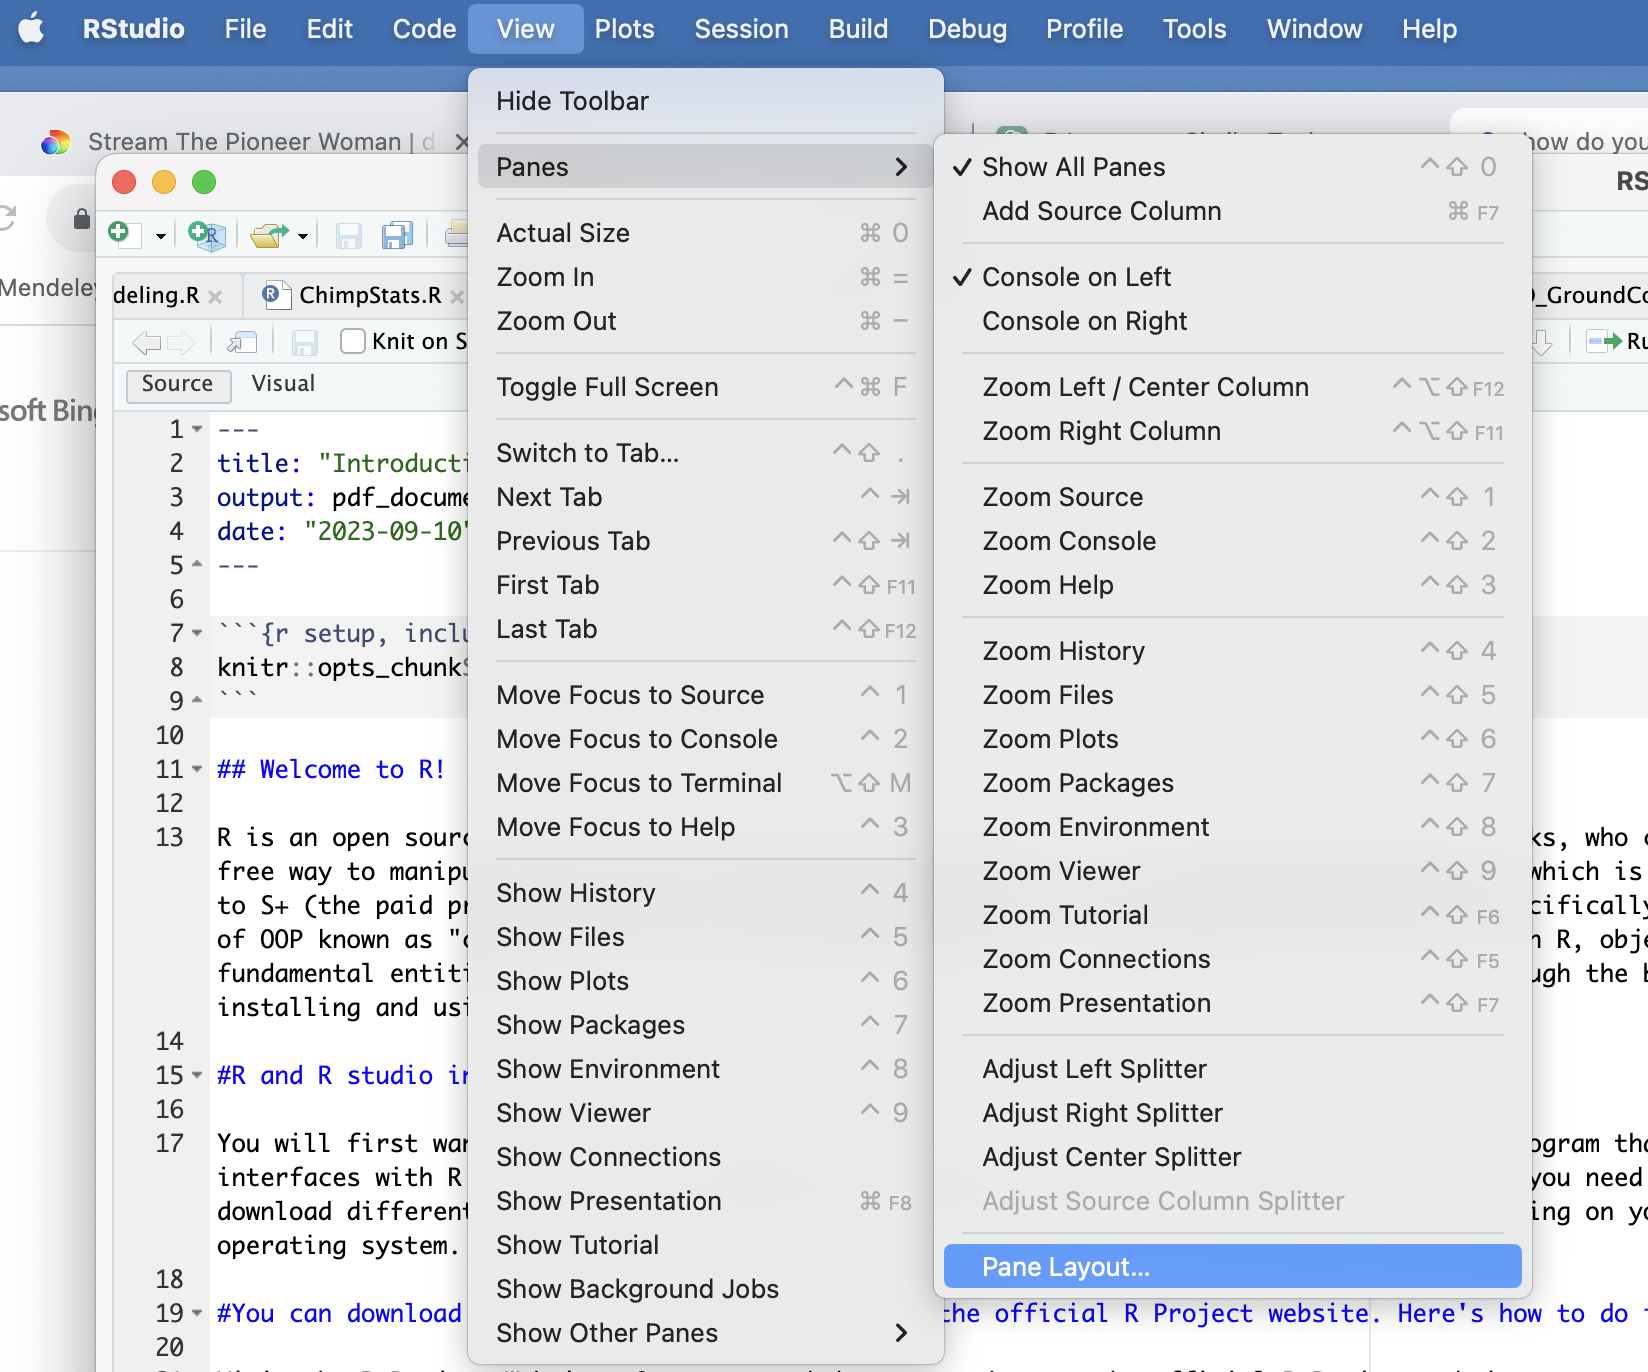
\includegraphics{/Users/sks379/Desktop/ENV226LabRManual/images:/01-intro/PaneLayout.png}

\hypertarget{good-housekeeping}{%
\section{Good housekeeping}\label{good-housekeeping}}

When you are coding in R, you will want to save your R or R markdown scripts and any other data files (e.g., .csv or spatial files) that you are analyzing in a common file. With good housekeeping, you will be able to seamlessly rerun your analyses at in point in time, allowing you to pick back up on projects that may have been dormant!

The first step in good R housekeeping is to set a \textbf{working directory}. A working directory tells R where to look for and save files. As an example, let's say I am planning to save everything associated with this tutorial to a file called Class1\_IntroToR. To do this, create a new folder on your desktop called `R is great'. You can change your working directory using the R studio interface by selecting a working directory at the top of the console panel in the ``Files'' tab. If you want to change your working directory to a different location, click on the ``\ldots{}'' (ellipsis) button in RStudio's ``Files'' tab. This will allow you to browse your file system and select a new directory as your working directory. That said, you will be \emph{far} better served by including code in your R script that directs R to your working directory. I prefer to set it within the code in order to allow you to instantaneously be able to pick up work where you left off rather than searching through files and trying to remember how you set up the code. You can view your working directory by running a simple bit of code (run code below).

\begin{Shaded}
\begin{Highlighting}[]
\FunctionTok{getwd}\NormalTok{() }\CommentTok{\#display file path to R studio }
\end{Highlighting}
\end{Shaded}

\begin{verbatim}
## [1] "/Users/sks379/Desktop/ENV226LabRManual"
\end{verbatim}

When you run, getwd() you will see where R is looking for files. Now, let's tell R where we want it to access files from! First, you will need to identify your file path. To find the file path to the Class1\_IntroToR on a mac, double click on the file and should see several option, including `Get info' (check out picture below).

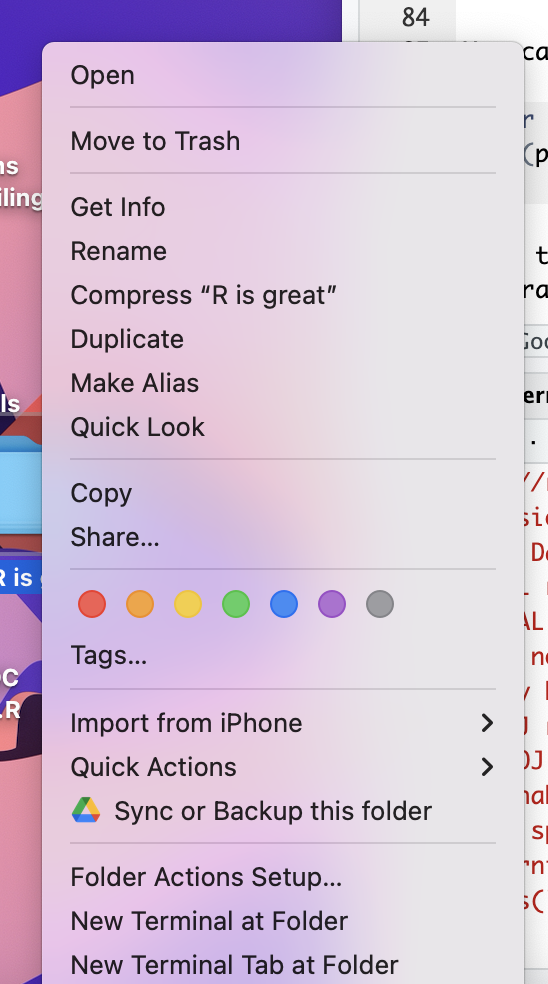
\includegraphics{/Users/sks379/Desktop/ENV226LabRManual/images:/01-intro/workingdirectorymac.png}

Then, select `Get info'. Then, highlight the information after `where' and copy it as a pathname (see picture).

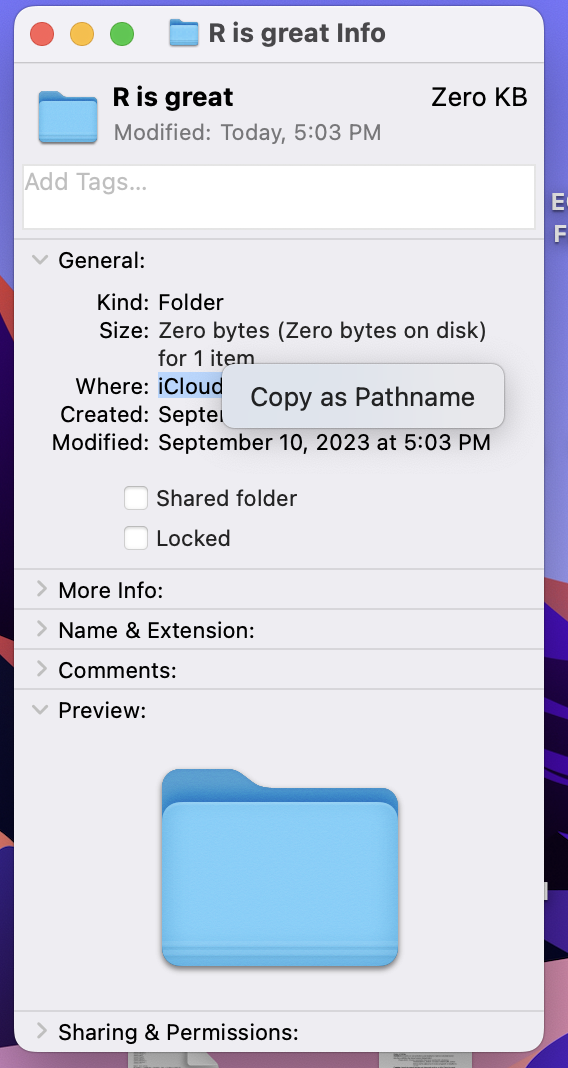
\includegraphics{/Users/sks379/Desktop/ENV226LabRManual/images:/01-intro/copyingpathnamemac.png}

For PCs, start by opening your File Explorer:
Press the Windows key + E on your keyboard.
Alternatively, you can click the ``File Explorer'' or ``This PC'' icon on your taskbar or Start menu.
Navigate to the Folder: Use the File Explorer to navigate to the folder where the file is located. You can click on folders to open them and view their contents.

\begin{enumerate}
\def\labelenumi{\arabic{enumi}.}
\item
  Find the File: Locate the file you are interested in within the folder.
\item
  View the File Path: Once you've found the file, you can see its full file path in the address bar at the top of the File Explorer window. The file path will be displayed as a sequence of folder and file names separated by backslashes. You can click in the address bar and copy the file path to the clipboard by pressing Ctrl + C after selecting it.
\item
  Once you have copied your file path, paste that path name into the following code and set your working directory: setwd(``/Users/sks379/Desktop/R is great/'')
\end{enumerate}

Now R studio is directed to upload and save work to this folder.

\hypertarget{annotating-your-code}{%
\section{Annotating your code}\label{annotating-your-code}}

Notice anything about the code in the section you just ran? You can use the hast tag symbol to tell R not to run a section of code. Whenever I am generating code, I try to add lots of notes to myself, so that that future me knows what code I created and why. Annotating your code is just good practice for coding! Alternatively, you can create R markdown files (what this tutorial has been created in), but R markdown, while generating pretty PDFs and websites, adds an extra layer of complexity that you generally don't want or need while coding, so I typically recommend creating an R script and annotating your that file! One thing that you might want to include in your code description is the version of R that you are using (you may need to load older versions of R if your scripts stop working due to updates to the program). To check the version of R that you are using, paste this in the command line: R.version.string

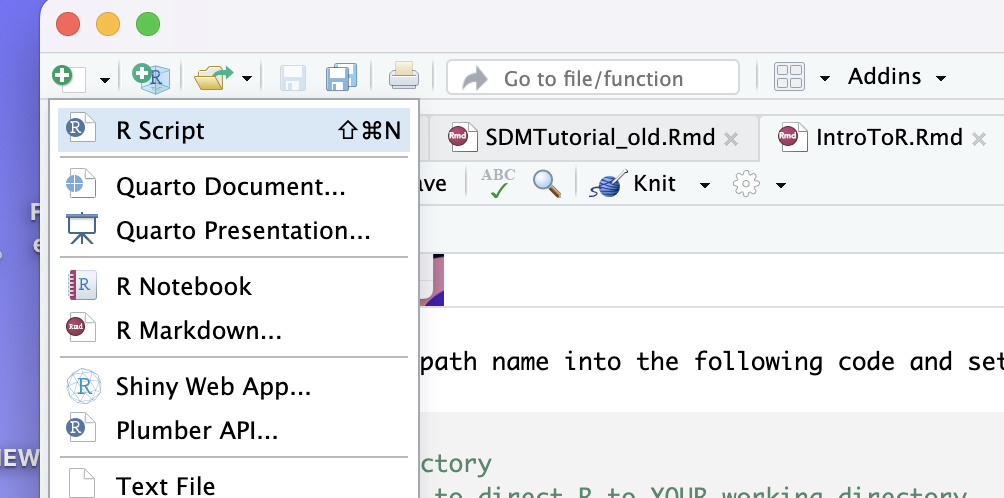
\includegraphics{/Users/sks379/Desktop/ENV226LabRManual/images:/01-intro/createrscript.png}

\hypertarget{libraries}{%
\section{Libraries}\label{libraries}}

Base R, the fundamental, built-in set of functions, data structures, and libraries that come with the R programming language without the need for additional packages or extensions, including basic math functions, statistical analyses and visualization tools. However, one amazingly cool think about R is that folks are out there creating `libraries', or a collection of R functions, data sets, and documentation bundled together into a single package, to do specialized analyses. For most tasks in R, you will need to install and load libraries. There are two methods to install libraries. Let's start by installing an important library (or package) for data manipulation, called `tidyverse' (actually several packages - hence why the name references a universe). To do this, run this code: install.packages(``tidyverse'').

The weird thing about including install packages code is that you don't want to re-install packages every time that you use R (in fact, it caused my R markdown code to freak out, which is why I've included the install function in the text). You will need to load packages, but you update R and R studio, you won't need to install packages after you have done it once. You can either then install the packages and delete the install code OR you can install through the R studio interface by going to packages, selecting install and searching for and installing the packages that you are interested in. When prompted, be sure to install dependencies - this will make sure that you have any pieces of code that the library that you are installing needs to operate.

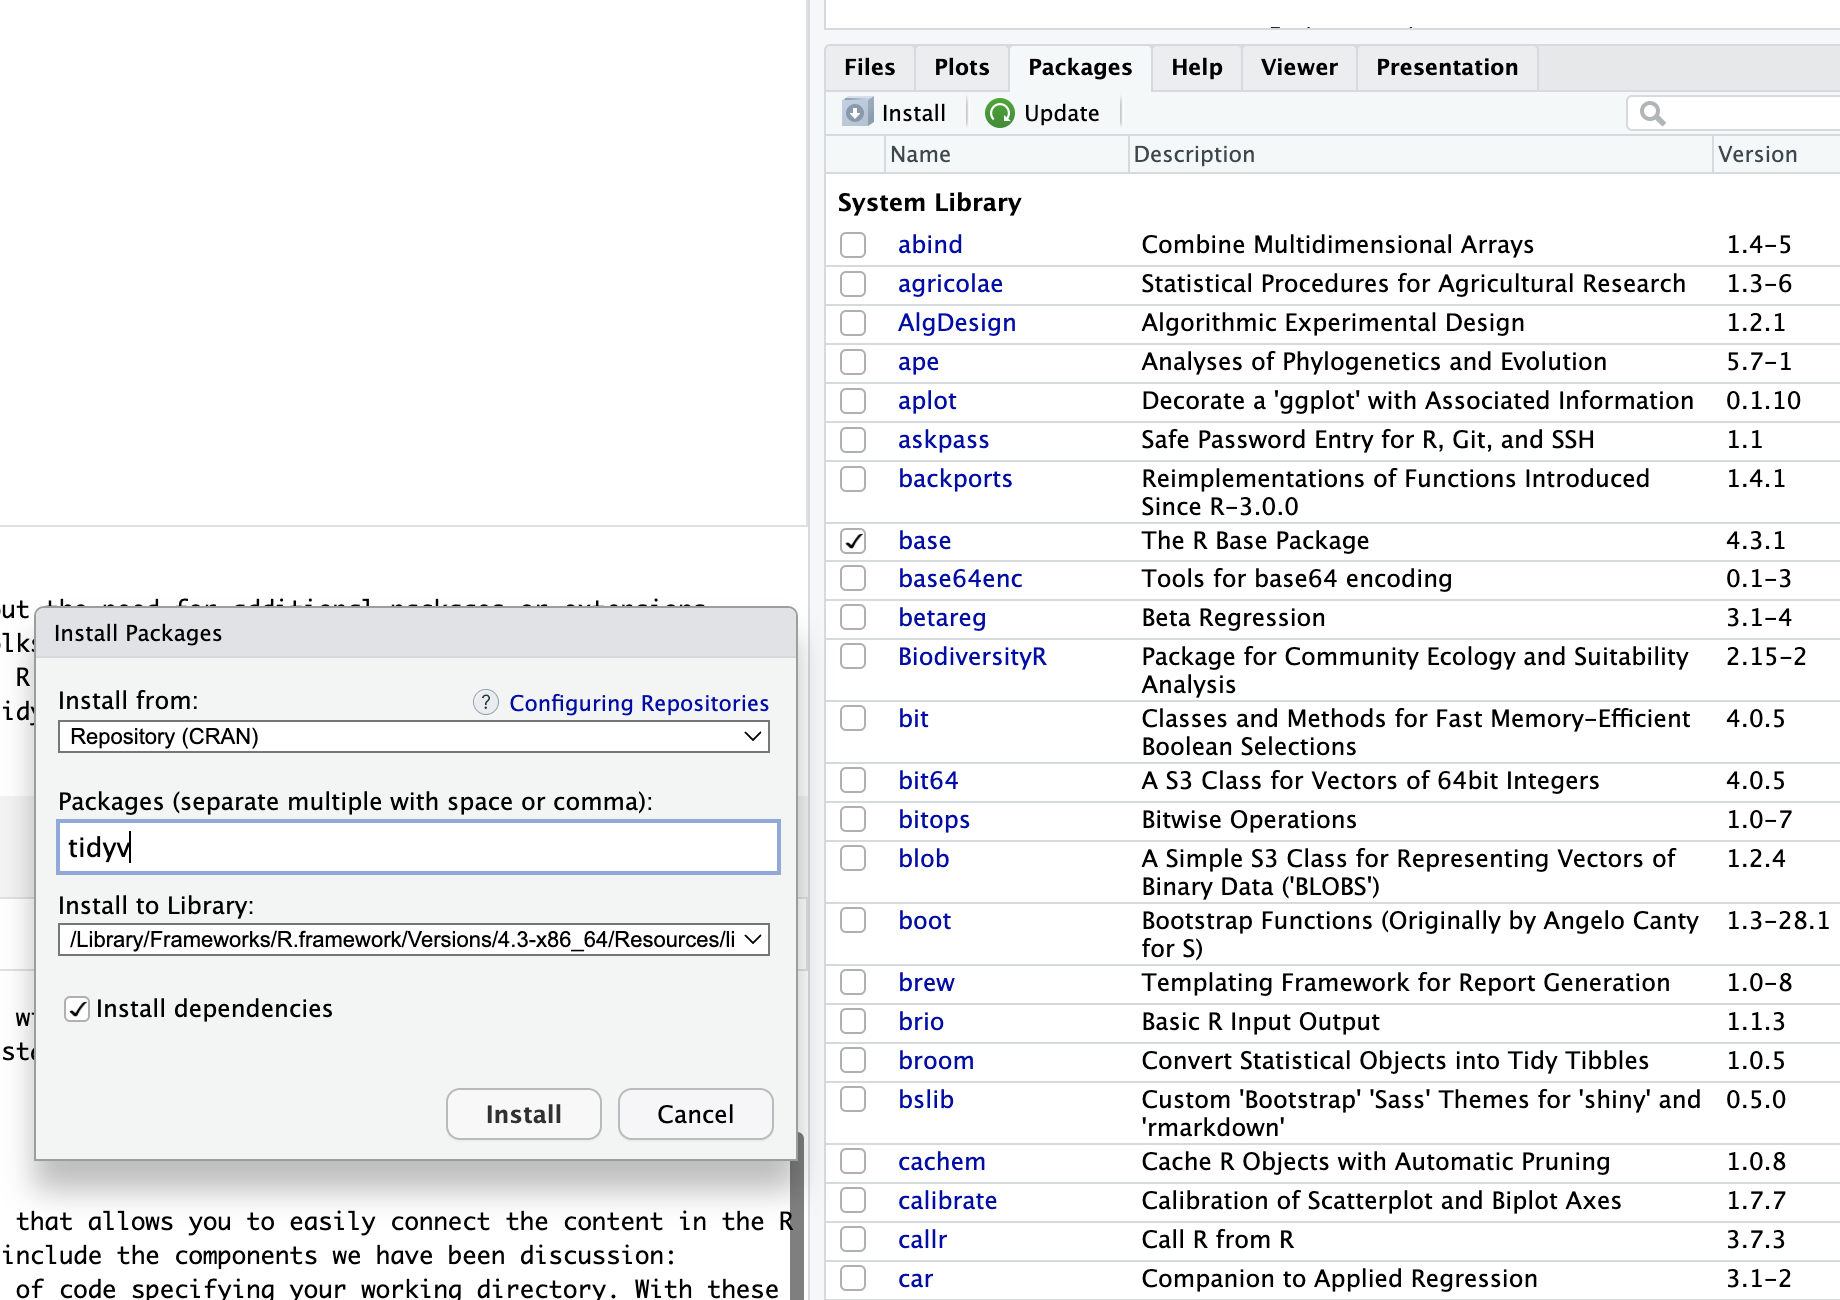
\includegraphics{/Users/sks379/Desktop/ENV226LabRManual/images:/01-intro/installlibraries.png}

Excellent! You have installed a library! Now, we need to load it. AND you will need to load R packages everytime that you use R. Any functions associated with your package won't work, unless the package is loaded, so I suggest keeping the load library code in your R script. The code is simple (see below).

\begin{Shaded}
\begin{Highlighting}[]
\FunctionTok{library}\NormalTok{(tidyverse)}
\end{Highlighting}
\end{Shaded}

Wonderful, you now have the essential knowledge base that you need to start working efficiently and effectively in R!

\hypertarget{organizing-your-code}{%
\section{Organizing your code}\label{organizing-your-code}}

A well-written R script will include the components we have been discussion: Annotated notes on what the script is doing and potentially even the version of R, loading commands for your libraries, and a line of code specifying your working directory. With these elements in place, you are ready to code your heart out!

Here is a glimpse at what your R scripts should look like.
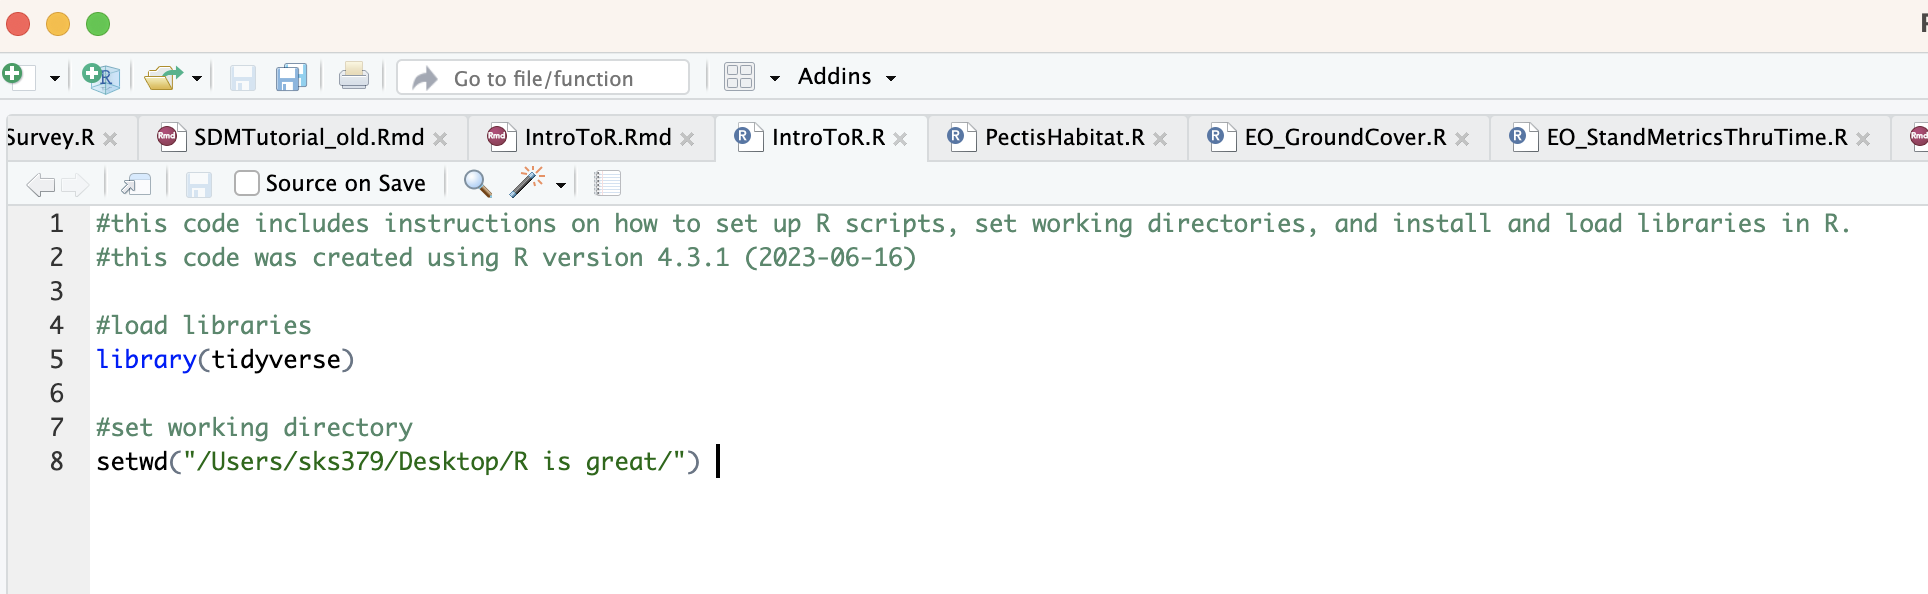
\includegraphics{/Users/sks379/Desktop/ENV226LabRManual/images:/01-intro/RScriptSetUp.png}

And with that, welcome to the wonderful world of coding in R!

  \bibliography{book.bib,packages.bib}

\end{document}
